% Copyright (c)  2005-2010 EDF-EADS-PHIMECA.
% Permission is granted to copy, distribute and/or modify this document
% under the terms of the GNU Free Documentation License, Version 1.2
% or any later version published by the Free Software Foundation;
% with no Invariant Sections, no Front-Cover Texts, and no Back-Cover
% Texts.  A copy of the license is included in the section entitled "GNU
% Free Documentation License".
\renewcommand{\filename}{docUC_InputBayesian.tex}
\renewcommand{\filetitle}{UC : Creation of a random vector with random parameters}

% \HeaderNNIILevel
% \HeaderIILevel
\HeaderIIILevel



\index{Distribution!Bayesian}
\index{Bayesian! Distribution}

The objective of this Use Case is to create and generate some realizations of a random vector $\vect{Y}$ which distribution $\mathcal{L}(\vect{\Theta})$ has random parameters $\vect{\Theta}$ distributed according to the distribution $\mathcal{D}_{\vect{\Theta}}$.\\

Note that the random parameters vector $\vect{\Theta}$ is a {\itshape RandomVector} object that can be :  
\begin{itemize}
  \item a {\itshape UsualRandomVector} which means described by a given distribution $\mathcal{D}_{\vect{\Theta}}$,  
  \item or a {\itshape CompositeRandomVector} which means the output vector of a fonction $f$ evaluated on the random vector $\vect{X}$  : $\vect{\Theta} = f(\vect{X})$. In that case, the distribution $\mathcal{D}_{\vect{\Theta}}$ is not explicitely known.
\end{itemize}

To generate a realization of such a random vector $\vect{Y}$, Open TURNS first generates a realization $\vect{\theta}$  of the random vector  $\vect{\Theta}$ according to  $\mathcal{D}_{\vect{\Theta}}$ then a realization of the distribution $\mathcal{L}(\vect{\theta})$ where the random vector $\vect{\Theta}$  is fixed to the previous realization $\vect{\theta}$ .\\

Details on each object may be found in the User Manual  (\href{OpenTURNS_UserManual_TUI.pdf}{see User Manual - Probabilistic Modeling / Random Vector}).\\



\requirements{
  \begin{description}
  \item[$\bullet$] the distribution $\mathcal{L}(\vect{\Theta})$   : {\itshape myYdist}
  \item[type:] Distribution
  \item[$\bullet$] the distribution $\mathcal{D}_{\vect{\Theta}}$   : {\itshape myThetaDist}
  \item[type:] Distribution
  \item[$\bullet$] the function $f$ : {\itshape myFunc}
  \item[type:] NumericalMathFunction
  \item[$\bullet$] the input random vector $\vect{X}$ : {\itshape inputXRV}
  \item[type:] RandomVector
  \end{description}
}
{
  \begin{description}  \item[$\bullet$] the random vector $\vect{\Theta}$: {\itshape  myThetaRandomVector}
  \item[type:]  RandomVector (of type Usual or Composite)
  \item[$\bullet$] the random vector $\vect{Y}$: {\itshape YrandomVector, rdTheta}
  \item[type:]  ConditionalRandomVector
  \item[$\bullet$] a distribution   : {\itshape Ydist }
  \item[type:] Distribution
  \item[$\bullet$] a random vector   : {\itshape rdTheta }
  \item[type:] RandomVector
  \end{description}
}

\textspace\\
Python script for this UseCase :

\begin{lstlisting}
  # First , create the random vector associated to the theta distribution

  # Case 1 : the distribution of theta is explicitely known
  # we create the random vector from the distribution
  myThetaRandomVector = RandomVector(myThetaDist)

  # Case 2 : the random vector Theta is the result of f(X)
  # and has been already defined previoulsy in the study
  # from a command such as 
  myThetaRandomVector = RandomVector(myFunc, inputXRV)


  # Then create the conditional random vector Y
  YrandomVector = ConditionalRandomVector(myYdist, myThetaRandomVector)

  # Generate some realizations of the conditional random vector Y
  N = 1000
  sampleY =   YrandomVector.getNumericalSample(N)

  # Get the distribution L(theta)
  Ydist =  YrandomVector.getDistibution()

  # Get the random vector theta
  rdTheta =  YrandomVector.getRandomParameters()

  # Get the dimension of L(theta)
  dimY =  YrandomVector.getDimension()  
\end{lstlisting}
\textspace\\

The following example illustrates a scalar random vector $Y$ distributed according to a Normal distribution $Normal(\mu, \sigma)$, parameterized as follows : 
\begin{itemize}
  \item the mean $\mu$ is distributed according to the Uniform distribution $Uniform([0,1])$,
  \item the standard deviation $\sigma$ is distributed according to the Exponential distribution $Exponential(\lambda=4)$.
\end{itemize}

The figure Fig.\ref{DensitCond} draws the probability density function of $Y$ that has been built with the kernel smoothing technique from $n=10^6$ realizations of $Y$ with the normal kernel. It also draws, for comparison needs, the probability density function of $Y$ in the case where the parameters are fixed to their mean value.\\



\begin{figure}[H]
    \begin{center}
      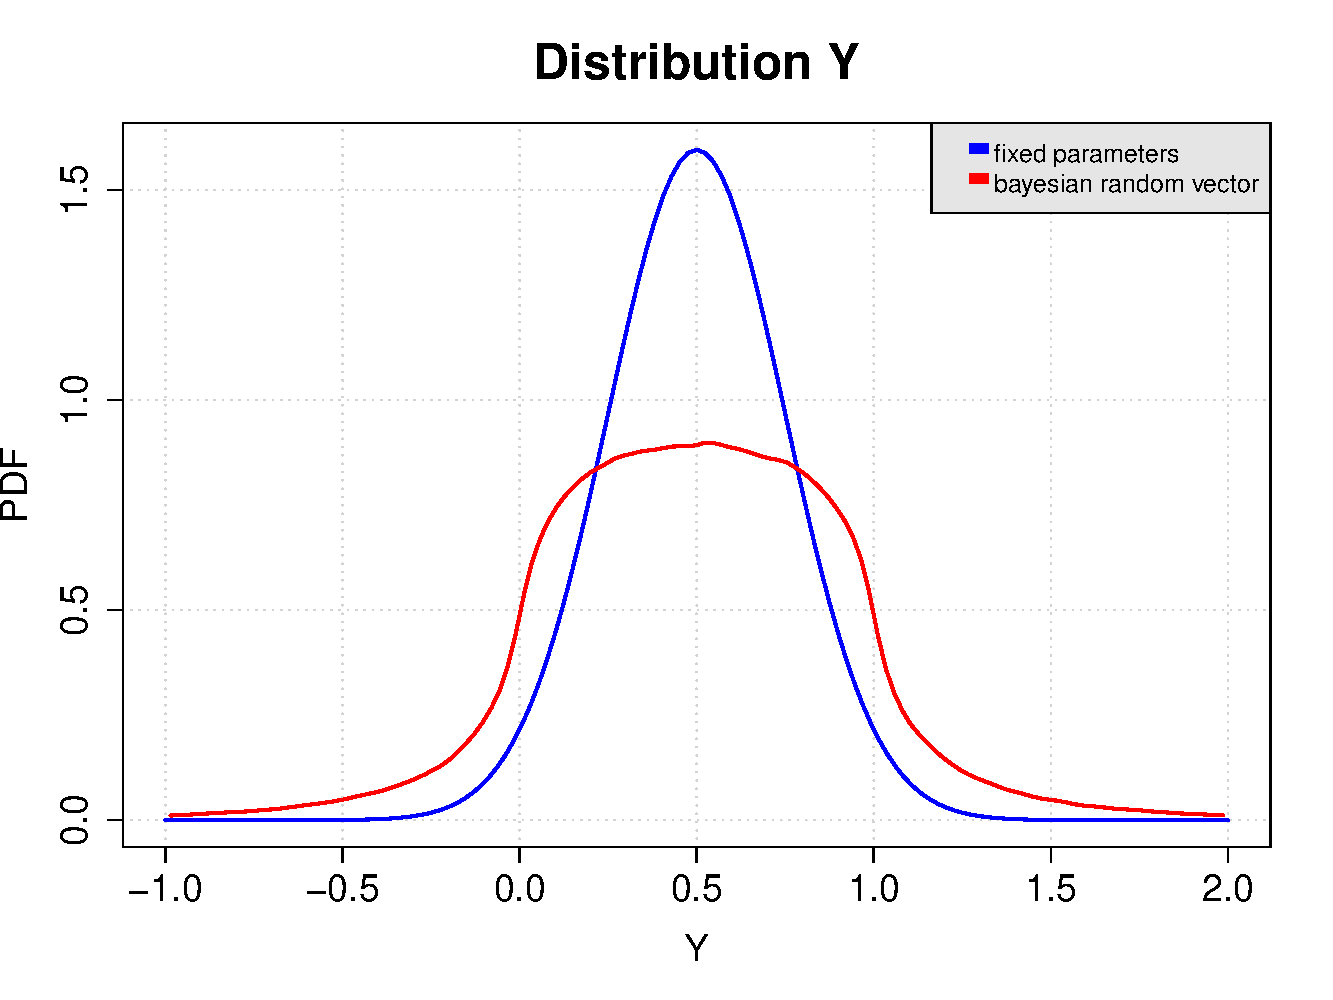
\includegraphics[width=7cm]{pdf_bayesianRandomVector.pdf}
      \caption{Normal distribution with random or fixed parameters.}
      \label{DensitCond}
    \end{center}
\end{figure}




Besides, if we consider the event $\mathcal{E} = \{Y > 1.5\}$, we have $Prob(\mathcal{E})= 1.75\, e-2$ in the first case of random parameters and $Prob(\mathcal{E})= 3.17\, e-5$ in the case of fixed parameters.
